\section{Introduction}
\label{sec:intro}



% Goal
Storage systems is the foundational platform for modern Internet services. Ever increasing reliance on massive data sets has forced developers to move towards a new class of scalable storage systems known as NoSQL key-value stores (KV-store). Most distributed NoSQL KV-stores (e.g., Cassandra \cite{Cassandra}, Riak \cite{Riak}, Dynamo \cite{Dynamo}) support a flexible data schema and simple GET/PUT (or Read/Write) interface for reading and writing data items. 
The data items are replicated at multiple servers to provide high fault-tolerance and availability. 

One drawback of the replication-based approach is the high storage cost. Erasure coding (EC) has been integrated with other types of KV-store to reduce storage cost (e.g., DepSky \cite{DepSky13} for cloud-of-clouds, Cocytus \cite{Cocytus2016} for in-memory KV-store  and Giza \cite{GIZA2017} for cross-datacenter KV-store).
This work is motivated by the following question: \textit{is it possible to use erasure coding in a NoSQL KV-store to reduce storage cost while maintaining strong consistency with moderate performance penalty?} We provide an affirmative answer by introducing \textbf{CassandrEAS (Cassandra + Erasure-coding Atomic Storage)}, a customized version of Cassandra \cite{Cassandra} with a new EC-based storage protocol that achieves \textit{atomicity} \cite{lamport}, a form of strong consistency. 

In this paper, we first present a novel quorum and erasure-code-based and storage cost optimized protocol called Two-Round Erasure coded Atomic Storage-Optimized (\treasmod{}). In addition to the improved storage cost, when compared to the existing erasure-code based algorithms, \treasmod{} algorithm is simple to implement as the high-level structure of the algorithm is very similar to the classic replication-based algorithm by Attiya, Bar-Noy and Dolev ~\cite{ABD96} and practical quorum storage ~\cite{Dynamo,pbs-vldb2012}. \treasmod{} is a two-round protocol that uses logical timestamps, which obviates the reliance on  any physical (machine) clock to implement atomic KV-store. We also modify \treasmod{} to use physical timestamp that results in a single-round distributed storage protocol One-Round Erasure coding Atomic Storage (\oreas). Both algorithms are suitable for quorum-based KV-store.%, and we replace  Cassandra's replication  mechanism  by  our EC-based  protocols.



\paragraph*{Cassandra}

% why Cassandra? why Strong consistency? what properties?
We chose to develop our system on top of Cassandra. Even though Cassandra was released in 2008, it is still one of the most used NoSQL KV-stores in industry. It is also an active open-source project (recent stable release in February 2020) \cite{DBEnginesCassandra}. Plus, its quorum-based replication \cite{pbs-vldb2012} shares similarly with other popular systems like Riak \cite{Riak} and Dynamo \cite{Dynamo}. For many big data applications, Cassandra offers a good balance of properties, e.g., high availability, scalability, and tunable consistency. Our system CassandrEAS provides similar guarantees in scalability and availability.%, because we aimed to integrate our protocol with Cassandra seamlessly (as will become clear later).


Cassandra offers tunable consistency guarantees, ranging from eventual consistency to strong consistency.
Popular storage systems in industry, such as Google Spanner \cite{Spanner} and CockroachDB \cite{cockroachDB}, are focusing on providing strong consistency. 
Inspired by the observation, this paper focuses on \textit{atomicity} \cite{lamport} (or linearizability \cite{herlihy1990linearizability}), one of the more popular forms of strong consistency, because atomicity is composable \cite{herlihy1990linearizability} and more intuitive for developing applications.

%Therefore, as the first step, CassandrEAS provides only atomicity.

Cassandra provides high availability and scalability using a quorum-based (or peer-to-peer) design.
It replicates data on multiple servers, and each server can serve any read/write request from clients 
using the practical quorum approach (or Dynamo-style quorum) \cite{pbs-vldb2012} for serving read and write operations. 
The approach does not use master node or consensus protocol to coordinate servers; hence, Cassandra has high performance without a single point of failure.\footnote{Cassandra  supports many operations beyond simple reads and writes, e.g., it uses Paxos \cite{paxos} to support transactions. Here we do not support transactions; we restrict its use to support only reads and writes, for which Cassandra does \textit{not} use Paxos (see Sec. \ref{s:CassandrEAS} for more detail).}  
Cassandra's quorum-based design make it difficult to use prior EC-based solutions \cite{Cocytus2016,GIZA2017,DepSky13}. Cocytus \cite{Cocytus2016} uses a master-based design, whereas Giza \cite{GIZA2017} is a consensus-based protocol. DepSky  \cite{DepSky13} does not provide atomicity. 

\subsection*{Main Contributions}
%\kishori{
%In this paper, we present a novel quorum and erasure-code-based and storage cost optimized protocol called Two-Round Erasure coded Atomic Storage-Optimized (\treasmod{}). \treasmod{} is a two-round protocol uses logical timestamps, which obviates the reliance on  any physical clock to implement the consistency guarantees. Based on this, we modify \treasmod{} to use physical clock that results in a single-round distributed storage protocol One-Round Erasure coding Atomic Storage (\oreas). The use of physical timestamps enables us to  implement \oreas{} into Cassandra \cite{Cassandra2010}, which uses physical timestamps, and we refer to our implementation as  CassandrEAS. More precisely, we replace Cassandra's replication mechanism by our EC-based protocol.}
In the theoretical contribution, we propose two novel EC-based atomic storage protocols: \treasmod{} and \oreas. From the engineering perspective, we demonstrate that our protocols can be seamlessly integrated with a real-world system, Cassandra. We made minimum modification to the original Cassandra codebase, and Cassandra users can call Cassandra's original read and write API directly \textit{without} knowing the details of the algorithm.
Our implementation can be found at \url{https://github.com/yingjianwu199868/cassandra/}
%To the best of our knowledge, this is the first implementation in NoSQL KV-Store that uses erasure coding.\footnote{We will release our code on Github once the paper is accepted in hope that stimulate more discussion and evaluation on using erasure codes in similar systems.} 

Using \treasmod{} and \oreas{}, CassandrEAS also provides availability and scalability at a similar level of Cassandra, because both systems do not use master or consensus.
One interesting feature of our protocols is a \textit{tunable knob} that allows clients to choose the desired level of availability (i.e., the maximum number of tolerated server failures), storage cost, and the number of supported concurrent operations. If there are more server failures or more concurrent operations than the specified parameters, then CassandrEAS may return stale value or fail to serve client's request. A protocol for self-stabilization, reconfiguration, or recovery is left as an interesting future work.

For evaluation, we deploy CassandrEAS in Google Cloud Platform (GCP) and conduct extensive experiments using the Yahoo! Cloud Service Benchamarking (YCSB) workload generator \cite{YCSB:2010}. YCSB is a practical tool used to benchmark many KV-stores.
%The implementation is discussed in Section \ref{s:implementation} and we present 
Our evaluation results in Section \ref{s:evaluation} indicate that CassandrEAS incurs moderate performance penalty, yet saves significant amount of storage space.

\paragraph*{Cassandra vs. CassandrEAS}
Table \ref{t:comparison} summarizes the comparison between Cassandra and CassandrEAS when storing one unit of data (i.e., data size is normalized to $1$). We do not count the size of meta-data such as timestamps. Erasure coding is more useful when dealing with larger data (say in terms of $100~B$s), so meta-data size is practically negligible. 
In the paper, $n$ denotes the number of servers that store the data, $\delta$ represents \underline{the maximum number of writes concurrent with any read on} \underline{the \textit{same} key-value pair}, and $f$ is the maximum number of tolerated crash servers.
For compactness, let $k = n-2f$. For Cassandra, we choose the majority quorum configuration.
% For Cassandra, we choose the quorum configuration. That is, both the read quorum and write quorum are of size $\frac{n}{2}+1$.

\begin{table}[h]
	\centering
	\begin{tabular}{ l|c|c|c}
		& Cassandra &  CassandrEAS  & \treas\\ \hline
		Storage cost/server & $1$ &  $\frac{1}{ \lceil\frac{k}{\delta+1}\rceil}$ 
		& $(\delta +1)\frac{1}{k}$ \\
	
		$f$, max crashes & $\frac{n}{2} - 1$  &  $\frac{n-k}{2}$ & $\frac{n-k}{2}$ \\%\hline
		%Read (Write) cost & $1$ &  $\frac{n}{ \lceil\frac{\delta+1}{k}\rceil}$\\\hline
	\end{tabular}
	\caption{Comparison of fault-tolerance level and storage-cost for Cassandra (Quorum), CassandrEAS and \treas}.
	\label{t:comparison}
	%\caption{Comparison of key performance metrics among the three implementations of strong consistency in Cassandra. $\delta$
	%	is the maximum number of writes concurrent with any read.}
	\vspace{-10pt}
\end{table}

In practical systems, the number of concurrent writes \underline{on the \textit{same} KV-pair} is small in most cases, since each operation completes in the order of $100~ms$. If CassandrEAS with $n=9$ is configured to tolerate $f=2$ crashed servers, and support $\delta = 3$ concurrent writes. In this case, $k = 5$, so the data storage cost at each server becomes
%\[
$\frac{1}{ \lceil\frac{k}{\delta+1}\rceil} = \frac{1}{ \lceil\frac{5}{3+1}\rceil} = \frac{1}{2}$.
%\]

In comparison, Cassandra's storage cost is $1$, as each server stores the original data. Hence, CassandrEAS saves $50 \%$ of storage space. If we have the configuration $n=7, f=1, \delta=1$, then $k=5$ and the storage cost of CassandrEAS is $\frac{1}{3}$, a $67\%$ reduction in storage space.

\remove{
\paragraph*{Our Contributions}
The main contribution of our paper is a new storage scheme for erasure coding based shared memory emulation algorithms. Our scheme has two benefits:
\begin{itemize}
	\item The storage cost of the new scheme is $\frac{B}{\lceil \frac{k}{\delta}\rceil}$ bits. Since $\frac{\delta}{k} \geq \frac{1}{\lceil \frac{k}{\delta}\rceil},$ note that the new storage scheme is at least as efficient as the usual erasure coding based storage scheme where each server stores codeword symbols for $\delta$ versions. \lewis{Cite something} \blue{just did} Furthermore, for certain parameters of $\delta,k$ the new scheme can be up to twice as storage-efficient as previous erasure coding based schemes~\cite{CadambeLMM17}. 
\item In the new scheme,  as in  the well-known replication-based algorithm by Attiya, Bar-Noy, and Dolev~\cite{ABD96} (which we refer to as ABD),  each node stores exactly one version of the data. This is contrast to previous erasure coding schemes, where $\delta$ versions of the data are stored at the server. From an implementation viewpoint, this could be beneficial as the server side code is essentially identical to ABD; only  the client side code should be modified as compared with repetition based schemes include encoding and decoding.
\item We modify \treasmod{} to use physical clocks present resulting in a single-round algorithm, (\oreas). 
We implement our protocols into Cassandra \cite{Cassandra2010}, namely CassandrEAS.
To the best of our knowledge, this is the first implementation in NoSQL KV-Store that uses erasure coding.
\end{itemize}
}
%\lewis{Do we really need these paragraphs? Doesn't seem very coherent with discussion before? Maybe move the first two paragraphs to the algorithm section?} \blue{removed them, you where right they are already explained in the algorithms}


% Our work
%We propose two new EC-based storage algorithms: a two-round algorithm, \treasmod{} (Two-Round Erasure coding Atomic Storage), using logical timestamp, and a one-round algorithm, \oreas{} (One-Round Erasure coding Atomic Storage), using physical timestamp. Both algorithms tolerate network asynchrony and crash failures of any client and some fraction of servers, and achieve \textit{near-optimal storage cost}. Each algorithm achieves slightly different guarantees and performance.
%Similar to the design of vanilla Cassandra, if clocks drift significantly, then \oreas{} might violate strong consistency. On the contrary, \treasmod{} ensures strong consistency at all time, but suffers an extra round of delay due to the usage of logical timestamp.


%\begin{figure*}[!ht]
%	\begin{subfigure}[b]{\columnwidth}
%		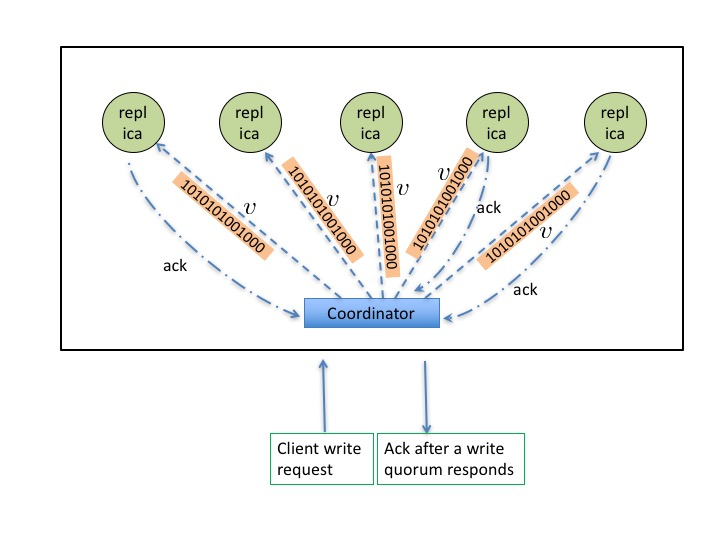
\includegraphics[width=\linewidth]{img/replication.jpg}
%		\caption{Cassandra stores the original value $v$.}
%		\label{fig:1}
%	\end{subfigure}
%	\hfill %%
%	\begin{subfigure}[b]{\columnwidth}
%		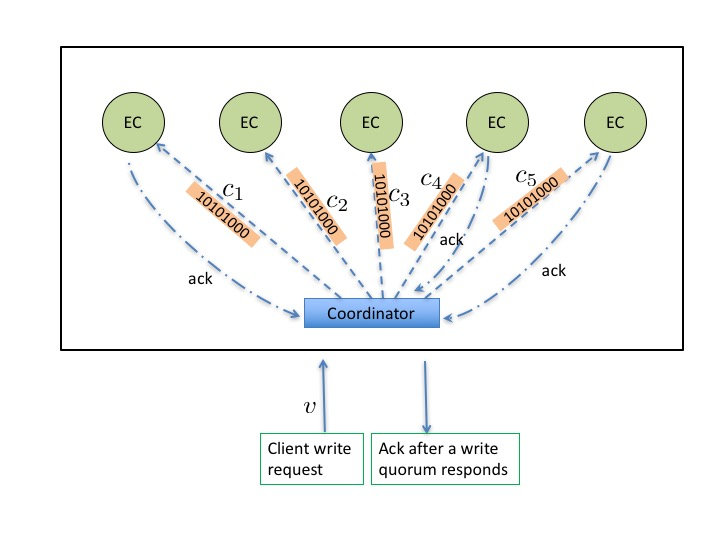
\includegraphics[width=\linewidth]{img/ec-code.jpg}
%		\caption{CassandrEAS only stores erasure-coded elements $c_i$'s.}
		%In TREAS and OREAS the erasure-coded elements of any value, e.g.,  $v$, is stored as  coded elements at separate servers.}
%		\label{fig:2}
%	\end{subfigure}
%	\caption{Illustration of Cassandra and CassandrEAS}
%\end{figure*}

% why EC?
% See motivaiton -- https://ipads.se.sjtu.edu.cn/_media/publications/cocytus_fast16.pdf
%\paragraph{Erasure Coding Storage Systems}
%\vspace*{3pt} \noindent \textbf{Erasure Coding Storage Systems}~~

